\documentclass[11pt,a4paper]{article}
\usepackage[utf8]{inputenc}
\usepackage[T1]{fontenc}
\usepackage{amsthm} %numéroter les questions
\usepackage[english]{babel}
\usepackage{datetime}
\usepackage{xspace} % typographie IN
\usepackage{hyperref}% hyperliens
\usepackage[all]{hypcap} %lien pointe en haut des figures
\usepackage[french]{varioref} %voir x p y
\usepackage{fancyhdr}% en têtes
%\input cyracc.def
\usepackage[]{graphicx} %include pictures
\usepackage{pgfplots}
\usepackage[]{circuitikz}
\usepackage{ifthen}

\usepackage[top=1.3 in, bottom=1.3 in, left=1.3 in, right=1.3 in]{geometry} % Yeah, that's bad to play with margins
\usepackage[]{pdfpages}

\usepackage[]{attachfile}

\usepackage{float}
\usepackage{subfig}

\usepackage{todonotes} % \missingfigure
\usepackage{gensymb} % \ohm

\usepackage{framed}

\newdateformat{mydate}{v2.0.0}%hack pour remplacer \THEYEAR


\newboolean{corrige}
\ifx\correction\undefined
\setboolean{corrige}{false}% pas de corrigé
\else
\setboolean{corrige}{true}%corrigé
\fi

%\setboolean{corrige}{false}% pas de corrigé

\newboolean{annexes}
\setboolean{annexes}{true}%annexes
%\setboolean{annexes}{false}% pas de annexes

\definecolor{darkblue}{rgb}{0,0,0.5}

\newboolean{mos}
%\setboolean{mos}{true}%annexes
\setboolean{mos}{false}% pas de annexes

\usepackage{aeguill} %guillemets

%% fancy header & foot
\pagestyle{fancy}
%Numero du TP :
\def \labonumber {Projet -- Part 1}
\lhead{[ELEC-H-310] Choucroute numérique\\ \labonumber}
\rhead{\mydate\today\\ page \thepage}
\chead{\ifthenelse{\boolean{corrige}}{Corrigé}{}}
\cfoot{}
%%

\pdfinfo{
/Author (ULB -- BEAMS)
/Title (\labonumber ELEC-H-310)
/ModDate (D:\pdfdate)
}

\hypersetup{
pdftitle={\labonumber [ELEC-H-310] Choucroute numérique},
pdfauthor={ULB -- BEAMS},
pdfsubject={}
}

\theoremstyle{definition}% questions pas en italique
\newtheorem{Q}{Question}[] % numéroter les questions [section] ou non []

\newcommand{\reponse}[1]{% pour intégrer une réponse : \reponse{texte} : sera inclus si \boolean{corrige}
	\ifthenelse {\boolean{corrige}} {\paragraph{Réponse :} \color{darkblue}   #1\color{black}} {}
 }

\newcommand{\addcontentslinenono}[4]{\addtocontents{#1}{\protect\contentsline{#2}{#3}{#4}{}}}

\date{\vspace{-1.7cm}\mydate\today}
\title{\vspace{-2cm}\labonumber \\ Digital electronics [ELEC-H-310]\\Design of an automatic fanning system: \\ pre-analysis and propeller fan power supply\ifthenelse{\boolean{corrige}}{~\\Corrigé}{}}

\setlength{\parskip}{0.2cm plus2mm minus1mm} %espacement entre §
\setlength{\parindent}{0pt}






\begin{document}
\pagestyle{empty}
\maketitle




\section*{Aims}
During the following three laboratory sessions, you will have to design a small cooling control system based on a propeller fan.
You will also have to be able to interact locally (through a keyboard) with this system.

During the first lab session, you will first pre-analyse the project in order to isolate the different features required by the project specifications.
Then, you will conceive the speed control of the propeller fan.

\section*{Prerequisite}
Before entering in the lab, you have to read the project specifications defined in the document ``Design of a temperature regulation system". You should also watch the tutorial on PWM on \url{https://www.cypress.com/video-library/PSoC-Software/psoc-101-lesson-8-pulse-width-modulator-pwm/387686}. 


\section*{Objectives}
At the end of this lab session, you'll be able to:
\begin{itemize}
	\item Slice a big amount of project specifications in submodules.
	\item Associate each module to the adequate peripheral devices.
	\item Generate a PWM wave and explain how it works.
\end{itemize}


\newpage




\section{Introduction}
During three laboratory sessions, you will have to design a small cooling control system based on a propeller fan.
You will also have to be able to interact locally (through a keyboard) with this system.

During the first lab session, you will first pre-analyse the project in order to isolate the different features required by the project specifications.
Then, you will conceive the speed control of the propeller fan.

The pre-analysis phase has a twofold objective : it helps to reinterpretate the project specifications with your words, as well as to push yourselves to slice the problem in simpler subproblems, with only for each a small amount of $\mu$C features.

Moreover, each of these submodule will be easy to reuse in other projects on condition that they are coded so that they are independent from each other.





\section{Preanalysis and reinterpretation of the project specifications}
To simplify the coding, you will first reinterpretate the specifications:
\begin{itemize}
	\item Generally speaking, what are the features required by the project specifications?
	Example: making the fan rotate at a controllable speed
	\item For each of these features, answer to the following questions:
	\begin{itemize}
		\item How does the interfacing with external world work?
		Must external circuits be added?
		\item What are the inputs and outputs?
		\item Which $\mu$C peripheral devices are used?
	\end{itemize}
	\item Realize a block diagram showing how those different features interact.
\end{itemize}






\section{Power supply and speed control of the propeller fan}
This first module that you have to implement is the speed control of the propeller fan, illustrated in figure~\ref{fig:helice}.

\begin{figure}[H]
\center
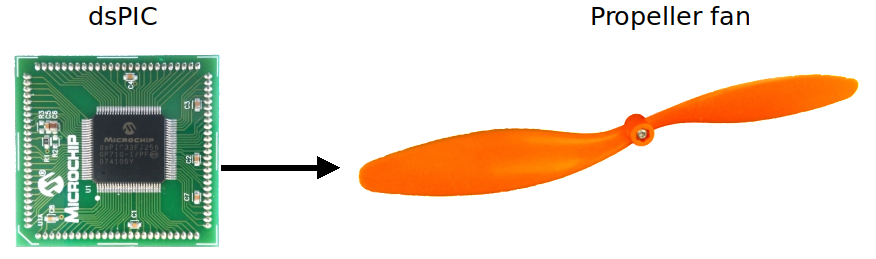
\includegraphics[width=0.8\textwidth]{alim-helice}
\caption{dsPIC33 controlling the propeller fan.}
\label{fig:helice}
\end{figure}

In order to do this, you will have to use the module named \textit{Pulse-Width Modulator (PWM)}, described in \url{https://www.cypress.com/video-library/PSoC-Software/psoc-101-lesson-8-pulse-width-modulator-pwm/387686}.

The principle of a PWM can be described as being a timer with two thresholds:
\begin{itemize}
	\item When the timer starts, the PWM output pin \texttt{pwm} is at ‘1’.
	\item When the counting register of the timer reaches the first threshold, named \texttt{CMP}, the output turns to ‘0’.
	The timer continues to increment.
	\item When the counting register reaches the value of the period \texttt{Period}, the timer returns zero and the output returns to ‘1’.
\end{itemize}
By playing with the values of \texttt{CMP} and \texttt{Period}, it is possible to generate any square wave.

Operational mode:
\begin{itemize}
	\item Instantiate a PWM in the TopDesign.cysch file. Configure it so you have a rectangular wave with a period of 100$\mu s$ and a duty cycle of 40\%. 
	\item Connect the output of the PWM to a pin on one of the jumpers J1 or J2 (see previous labs and ``Extension PSOC'' file). Verify your square wave with an oscilloscope. 
	\item By using the potentiometer and ADC code from the previous lab, modify your firmware (i.e. the main.c) so that the duty cycle of the PWM is changed when the potentiometer is turned. When the potentiometer is fully turned to one side, the duty cycle of the PWM should be 100\%. When the potentiometer is fully turned to the other side, the duty cycle of the PWM should be 0\%. 
	\item Connect the power supply pins of the propeller fan at 0V-5V of a protoboard, and connect the input In1 or In2 of the propeller fan to your PWM output.
	Do not forget to connect your grounds together!
	\item Check if the propeller fan rotates with a variable speed.
\end{itemize}






\section{PWM as a digital-to-analog converter}
The PWM modulation can be applied to the digital-to-analog conversion.


By eliminating the high frequency components with a decoupling capacitor, we only keep the mean value of the signal, that is to say $D(t) \cdot 5V$, where $D(t)$ is this evolution of the duty cycle over time\footnote{A variant of this principle, known as Delta modulation (or Sigma Delta), is used in analog-to-digital converters with high resolution and low frequency, as well as in the audio sector.}.

\begin{itemize}
	\item Using an oscilloscope, analyze the spectrum of the PWM signal.
	\item In this spectrum, observe the effect of the modulation.
	\item How to size the RC filter to eliminate the switching effect?
	\item Deduce the limits of this principle: can we convert any type of signal?
\end{itemize}


\end{document}
